\documentclass[letterpaper]{article}
\usepackage[submission]{aaai2027}
\usepackage{times}
\usepackage{helvet}
\usepackage{courier}
\usepackage[hyphens]{url}
\usepackage{graphicx}
\usepackage{booktabs}
\usepackage{microtype}
\usepackage{amsmath}
\usepackage{amssymb}
\usepackage{natbib}
\usepackage{caption}
\frenchspacing
\setlength{\pdfpagewidth}{8.5in}
\setlength{\pdfpageheight}{11in}
\urlstyle{rm}
\def\UrlFont{\rm}

\pdfinfo{
/TemplateVersion (2027.1)
}

\setcounter{secnumdepth}{0}

\title{Supplementary Material: Graph-Guided Mixture-of-Experts \\
for Unified Multimodal Mental Health Assessment}

\author{
Anonymous Authors
}
\affiliations{
}

\begin{document}

\maketitle

\section{Experimental Pipeline Overview}

The graph-routing investigation is one of the paper's supporting analyses (the main empirical question is the construct-bottleneck result, main paper Section~4). To isolate the routing effect, we compare five graph-routing ablation variants (V0--V4) against a non-graph baseline, across the 5 canonical seeds. We deployed a homophily diagnostic comparing real graph edges against random pairing, alongside two single-seed exploratory fixes: a $K$-sensitivity sweep ($K=5, 10, 15, 20$) and learning a per-task $\lambda$ weight instead of fixing it at 0.5. Under 5-seed, reportability-gated statistics, routing shows no distinguishable effect on DAIC or MOSEI, and a robust, directionally consistent degradation on FI personality despite FI carrying strong real graph signal by every measure we computed — the router's failure on FI is not signal absence, and the picture is more specific than a uniform "signal absent or unused" story (main paper, Section~4).

\begin{figure*}[htbp]
\centering
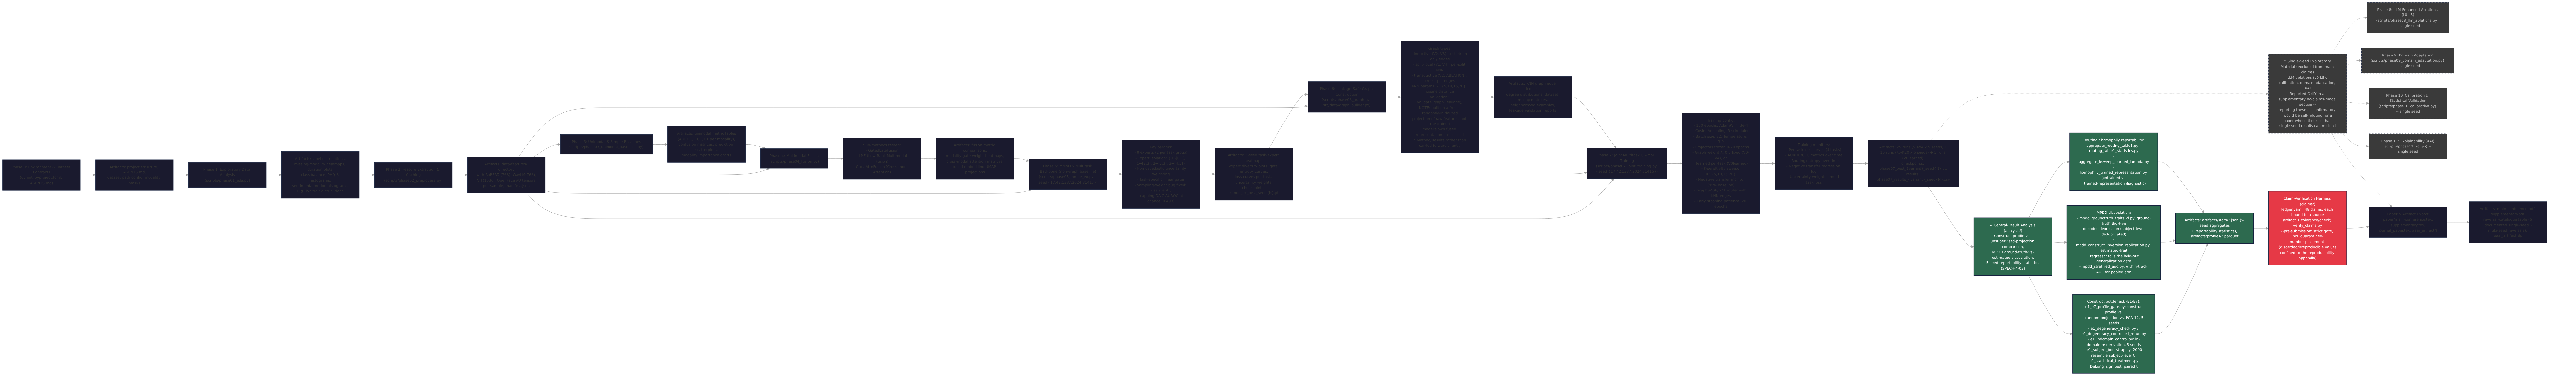
\includegraphics[width=0.85\textwidth]{figures/pipeline-flow.png}
\caption{Implementation detail of the experimental pipeline: the non-graph MMoEEx baseline (Phase 5) and the graph-routed joint multitask training (Phase 7) share the same DataLoader, initialization, and epoch training loop, differing only in whether the graph router contributes to expert routing; both feed the central-result analysis (construct-profile comparison, MPDD dissociation, 5-seed reportability statistics) and the claim-verification harness. LLM ablations, domain adaptation, calibration, and explainability (dashed) are single-seed exploratory material, excluded from the paper's claims.}
\label{fig:training_pipeline}
\end{figure*}

\section{Leakage Protocol Details}

\subsection{Graph Construction per Split}

For each dataset, we construct KNN graphs using one of three leakage-safe modes (see Section 3, ``Method,'' of the main paper):

\begin{itemize}
    \item \textbf{Inductive}: the graph is built on training-split embeddings only. Validation and test nodes connect exclusively to their $K$ nearest \emph{training} neighbours; they never connect to each other.
    \item \textbf{Split-local}: separate graphs are built independently for train, validation, and test. No edge crosses a split boundary.
    \item \textbf{Transductive} (ablation only, not leakage-safe): a single graph is built over all splits jointly, so validation/test nodes may connect to each other. Retained only to quantify how much a naive (non-leakage-safe) protocol would inflate results.
\end{itemize}

DAIC-WOZ: 189 sessions (107 train / 35 val / 47 test), subject-independent — no participant ID appears in more than one split. CMU-MOSEI and ChaLearn FI use their official utterance-/clip-level splits (see Section 3, ``Method,'' of the main paper). All splits are validated by an automated leakage audit (9/9 checks passing: inductive train/test, split-local val/test, transductive cross-split-edges-expected, bug-injection detection, and LLM-feature independence).

\section{Hyperparameters}

\begin{table}[t]
\centering
\caption{Complete hyperparameter configuration.}
\label{tab:hparams}
\small
\begin{tabular}{ll}
\toprule
Parameter & Value \\
\midrule
Common dimension $d$ & 256 \\
MMoEEx experts $M$ & 8 \\
Expert hidden size (both configurations) & 256 \\
GraphSAGE layers & 2 \\
GraphSAGE hidden size & 126 \\
GraphSAGE aggregation & Mean \\
GAT heads / head dim (ablation) & 3 / 42 \\
KNN neighbours $K$ & 10 or 15 (per variant) \\
Edge similarity metric & Cosine \\
Graph routing weight $\lambda$ & 0.5 (fixed, not tuned) \\
Learning rate & $3 \times 10^{-4}$ \\
Optimizer & AdamW \\
Batch size & 32 \\
Epochs (max) & 150 \\
Early stopping patience & 20 \\
Projector freeze epochs & 20 \\
Temperature balance $T$ & 3.0 \\
\bottomrule
\end{tabular}
\end{table}

\section{Complete Ablation Results}

\begin{table*}[t]
\centering
\caption{Full ablation ladder. Rows 0--1 are single-seed (not yet extended to the 5-seed protocol used elsewhere in this paper; flagged accordingly). Rows 2--5 report mean $\pm$ std over the 5 canonical seeds (17, 42, 1337, 2024, 31415).}
\label{tab:full_ablation}
\small
\begin{tabular}{llcccc}
\toprule
 & & DAIC AUROC & MOSEI Sent. CCC & MOSEI Emotion AUROC & FI Avg CCC \\
\midrule
0 & Trivial (majority class)$^\ddagger$ & 0.500 & 0.000 & 0.500 & 0.000 \\
1 & + Unimodal (best modality: text/text/video)$^\ddagger$ & 0.584 & 0.512 & --$^\dagger$ & 0.458 \\
2 & + MMoEEx (no graph) & 0.541 $\pm$ 0.017 & 0.482 $\pm$ 0.011 & 0.710 $\pm$ 0.005 & 0.571 $\pm$ 0.006 \\
3 & + KNN voting (no learned router) & 0.623 $\pm$ 0.071 & 0.428 $\pm$ 0.021 & 0.674 $\pm$ 0.013 & \textbf{0.373 $\pm$ 0.011} \\
4 & + Graph router (V0, inductive $K{=}10$) & 0.518 $\pm$ 0.027 & 0.510 $\pm$ 0.024 & 0.722 $\pm$ 0.009 & 0.480 $\pm$ 0.060 \\
5 & + Graph router (V3, inductive $K{=}15$) & 0.549 $\pm$ 0.057 & 0.501 $\pm$ 0.022 & 0.714 $\pm$ 0.014 & 0.507 $\pm$ 0.047 \\
\bottomrule
\end{tabular}

\vspace{2pt}
{\footnotesize $^\dagger$Per-modality unimodal baselines evaluate MOSEI emotion as a regression task (CCC per emotion, averaged); no per-modality classification AUROC was computed at the unimodal stage, so this cell is not directly comparable to the classification AUROC reported for rows 3--6 and is left blank rather than filled with an unrelated number. $^\ddagger$Single-seed; not yet extended to the 5-seed protocol.}
\end{table*}

Row 1's DAIC AUROC (0.584) is a same-protocol recomputation (nested-CV $\ell_2$-regularized logistic regression on the raw 768-dim RoBERTa embedding, identical train/test participants as every other DAIC number in this paper).

Rows 2--5 are averaged over the 5 canonical seeds. Under the 5-seed reportability rule (main paper, Section~4), none of the DAIC deltas between rows 2--5 are distinguishable from seed noise at $n{=}5$ — including row 3's apparent DAIC advantage over row 2 ($+0.083$, paired $p{=}0.087$, not reportable). Row 3 does, however, show a reportable, robust \emph{negative} delta from the non-graph baseline on all three other metrics (MOSEI sentiment CCC $p{=}0.003$, MOSEI emotion AUROC $p{=}0.014$, FI CCC $p{<}0.001$) — simple neighborhood label-smoothing is not a free lunch once measured across seeds, even though it happens to land numerically close to the DAIC baseline. FI personality is the one metric where the learned graph-router rows (4--5) also show a reportable, robust negative delta from the non-graph baseline (main paper Table~1; 3 of 5 variants significant at $p<0.05$, the other two borderline) — consistent with, not contradicted by, row 3's own FI degradation.

\paragraph{Fusion ablation (single-seed).} A single-seed fusion comparison (a separate isolated-fusion training run rather than the joint multitask pipeline used everywhere else in this paper) found cross-attention fusion below gated late fusion on DAIC AUROC (0.379 vs.\ 0.442) and MOSEI sentiment CCC (0.540 vs.\ 0.575); on FI, both fusion types collapsed to near-zero CCC in this isolated ablation and the comparison is uninformative there. This is reported here as single-seed and exploratory, rather than in the main paper's Results.

\section{Graph-Sensitivity Sweep}

\begin{figure}[t]
\centering
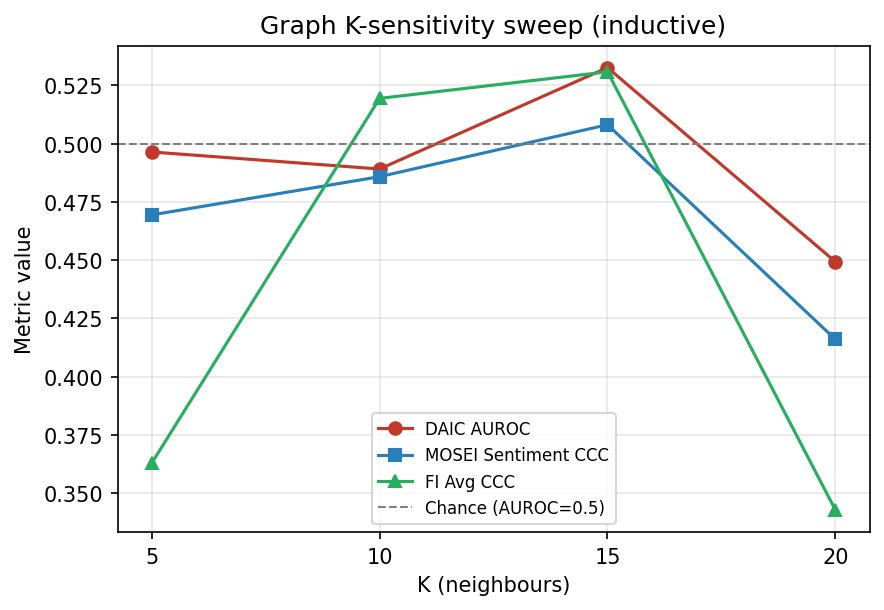
\includegraphics[width=0.9\columnwidth]{figures/k_sensitivity.png}
\caption{5-seed mean $\pm$ std, inductive graph: no monotonic trend with $K \in \{5,10,15,20\}$ ($K{=}10$, $K{=}15$ are V0/V3 above). DAIC AUROC: $0.541\pm0.048$ ($K{=}5$), $0.518\pm0.027$ ($K{=}10$), $0.549\pm0.057$ ($K{=}15$), $0.526\pm0.057$ ($K{=}20$) — none reportably different from the non-graph baseline ($0.541\pm0.017$) under this strict rule.}
\label{fig:k_sensitivity}
\end{figure}

$K{=}5$ shows a reportable, robust \emph{negative} FI CCC delta from the non-graph baseline ($0.467\pm0.074$ vs.\ $0.571\pm0.006$, paired $p{=}0.04$), consistent with the FI-degradation pattern in Table~1; $K{=}20$'s FI delta is borderline ($p{=}0.06$), matching V3/V4's borderline status at $K{=}15$.

\section{Learned Routing Weight}

\begin{figure}[t]
\centering
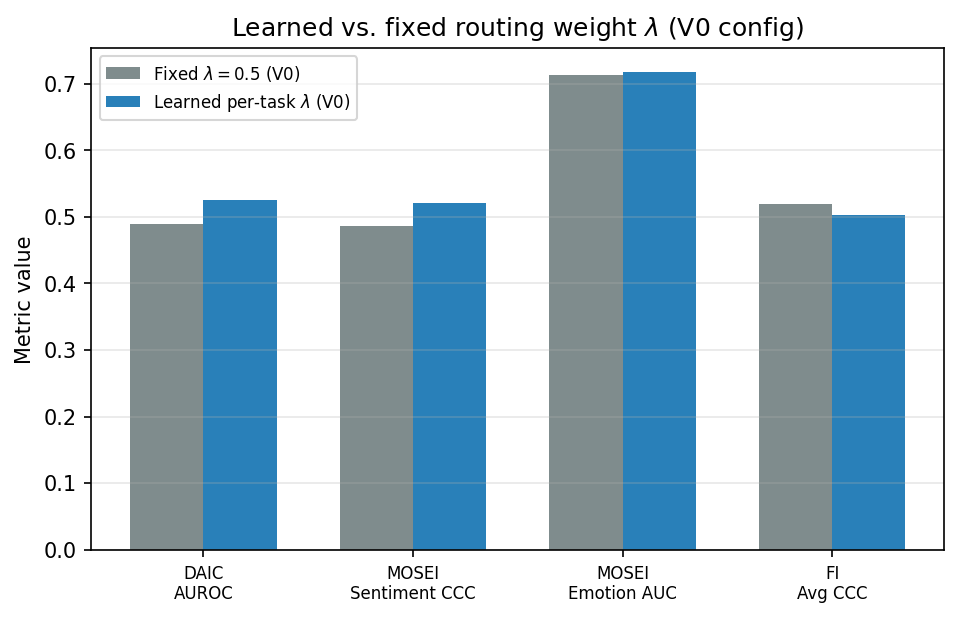
\includegraphics[width=0.9\columnwidth]{figures/learned_lambda.png}
\caption{5-seed mean $\pm$ std: learned per-task $\lambda$ (V0 configuration) reaches DAIC AUROC $0.546\pm0.034$ against the fixed-$\lambda{=}0.5$ V0 baseline's $0.518\pm0.027$ — a delta of $+0.028$ that is \textbf{not reportable} under the strict effect-size criterion, despite a naive paired $t$-test alone giving $p{=}0.007$. FI CCC moves from $0.480\pm0.060$ (fixed $\lambda$) to $0.501\pm0.047$ (learned), also not reportable.}
\label{fig:learned_lambda}
\end{figure}

\section{Additional Figures}

\begin{figure}[t]
\centering
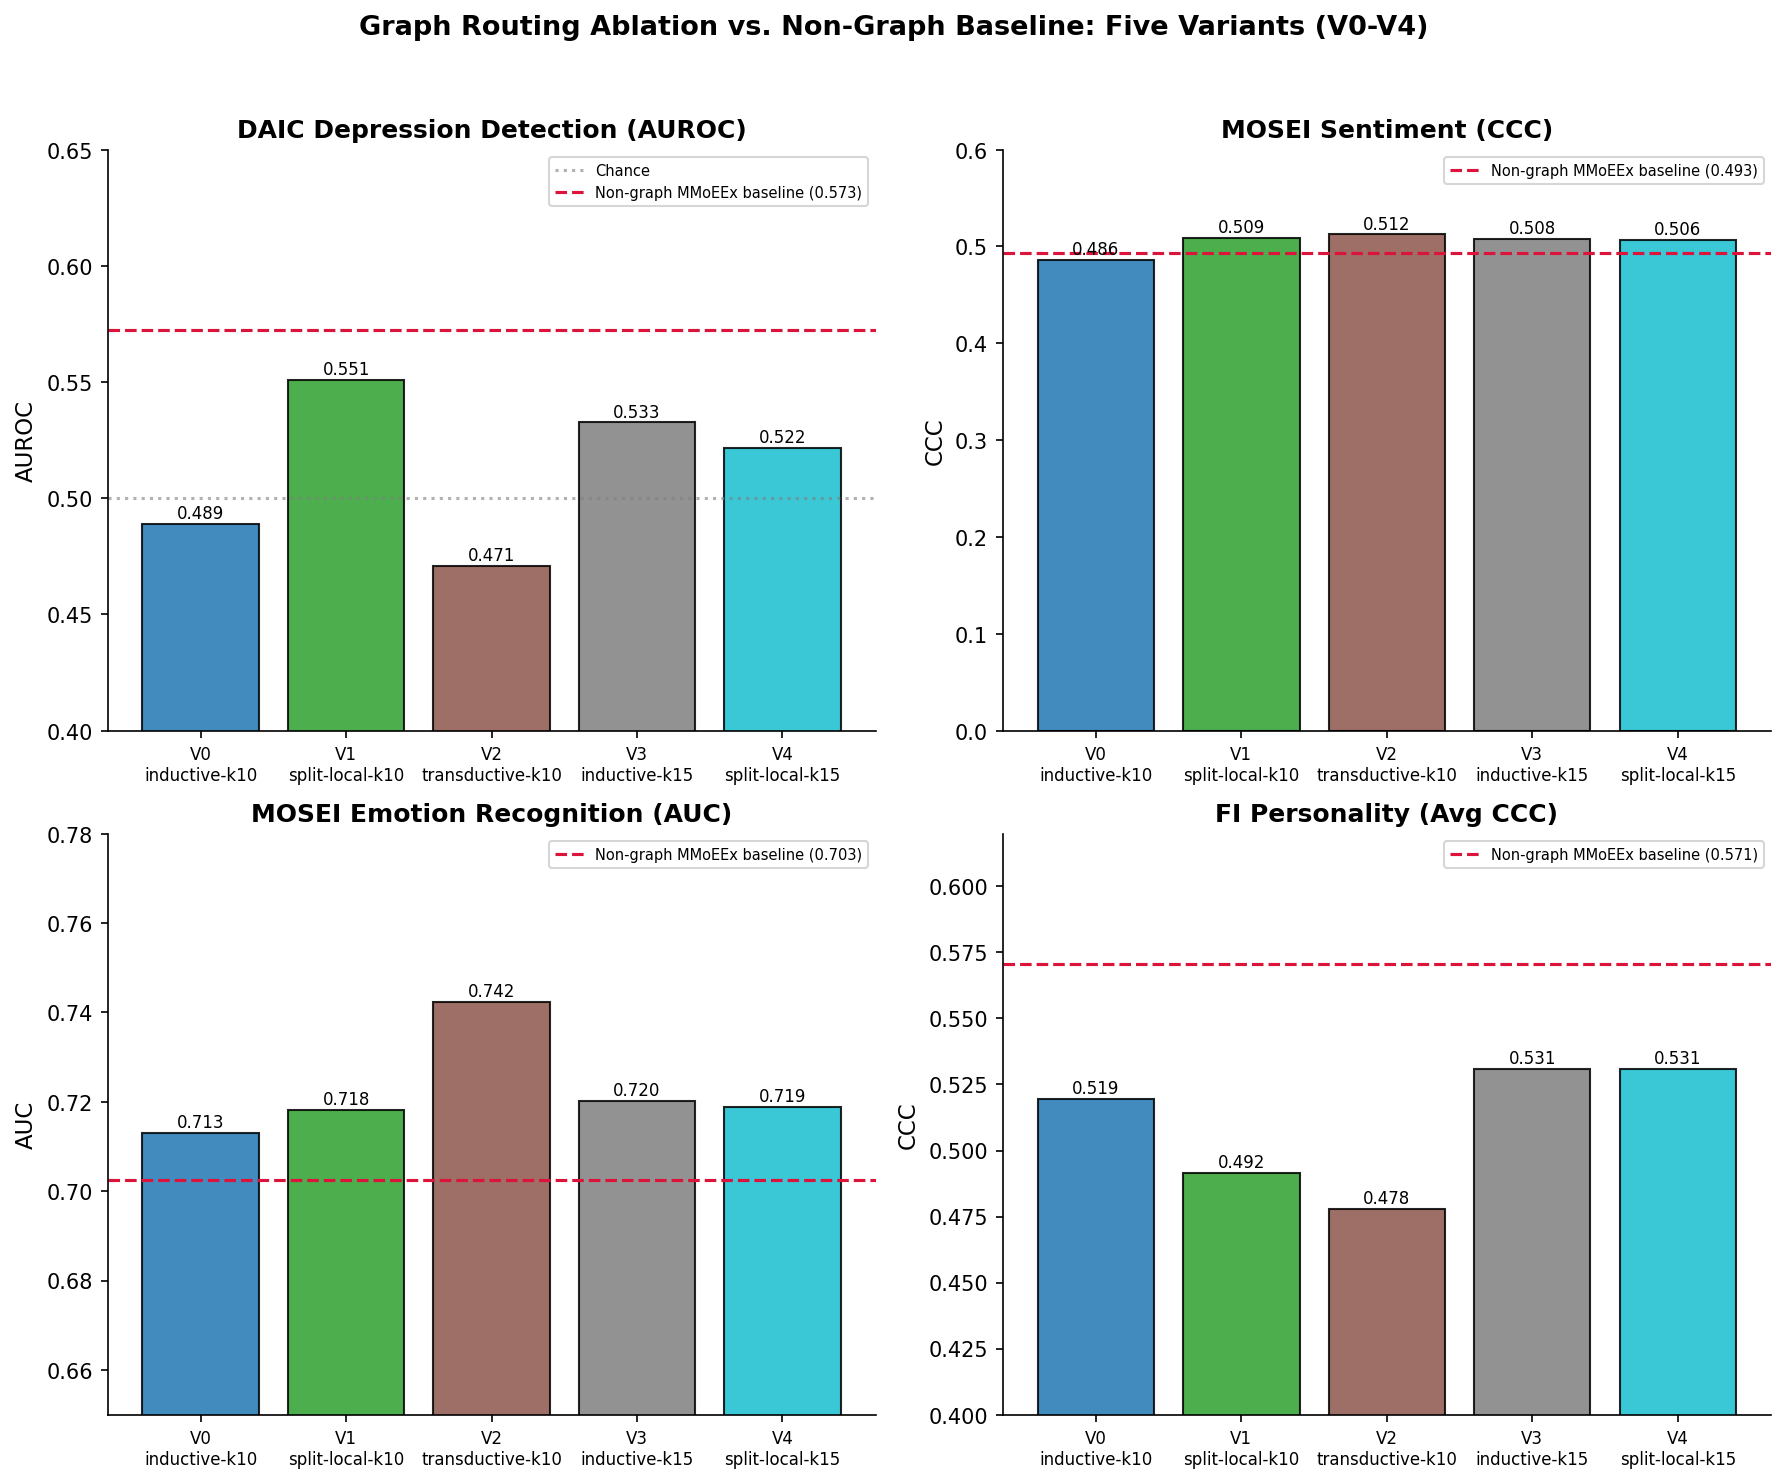
\includegraphics[width=0.9\columnwidth]{figures/graph_ablation.png}
\caption{Graph routing ablation vs.\ non-graph MMoEEx baseline (red dashed line), all five variants across all four tasks.}
\label{fig:graph_ablation_supp}
\end{figure}

\section{Single-Seed Exploratory Material: LLM Encoders, Calibration, Domain Adaptation, Explainability}
\label{sec:single_seed_exploratory}

\textbf{No claims are made from this section.} Every result below was run on a single seed, was never extended to this paper's 5-seed protocol, and touches none of the paper's three evidenced claims (the construct-projection inversion, the MPDD dissociation, or the localizability/homophily result). We include it because it was part of this project's development history, not because it supports or contradicts anything in the main paper. Table~\ref{tab:exploratory_summary} summarizes it; no number here should be cited as a finding.

\begin{table*}[t]
\centering
\caption{Single-seed exploratory results, not extended to this paper's 5-seed protocol, reported for development-history completeness only. None of these touch the main paper's evidenced claims.}
\label{tab:exploratory_summary}
\small
\begin{tabular}{p{0.22\textwidth}p{0.68\textwidth}}
\toprule
Analysis & Single-seed result (exploratory only) \\
\midrule
LLM-based encoders (L0--L5) & Replacing classical encoders with Mistral-7B/CLAP/LLaVA-1.5-7B: point-estimate gains on MOSEI (sentiment CCC $+0.140$, emotion AUROC $+0.064$), a gain on DAIC only from the full LLM stack ($+0.076$), and a loss on FI at every level. In the original single-seed analysis, no DAIC comparison against the classical baseline reached significance by the DeLong test (all $p>0.72$, $n{=}35$) — these were already reported as suggestive, not confirmed, before this paper's 5-seed protocol existed. \\
Post-hoc calibration & Temperature/Platt/isotonic scaling on the DAIC classifier (single LLM level): isotonic regression reduced ECE most (0.26--0.35 uncalibrated to lower after calibration); all three methods are monotonic and leave AUROC-based discrimination unchanged by construction. \\
Cross-dataset domain adaptation & CORAL/MMD/DANN/combined, transferring FI/MOSEI representations to DAIC: underperformed a no-adaptation baseline in 10 of 12 conditions, single seed. Separately, on the external MPDD benchmark (Wav2Vec2+OpenFace features, distinct from this paper's MPDD ground-truth-vs-estimated dissociation, main paper Section~4): a regularized logistic regression outperformed our architecture (AUROC 0.674 vs.\ 0.545--0.559); zero-shot Young$\to$Elderly transfer collapsed below chance (0.395); MPDD$\to$DAIC transfer was positive (0.551). \\
Explainability case studies & 9 case studies (3 per dataset) passing each sample through all four task heads, paired with SHAP/GNNExplainer/GraphXAIN-style post-hoc narratives. A faithfulness check (modalities outside a dataset's native routing show exactly zero attribution, 43/90 perturbation tests) held up; rebuilding the explanation graph on the model's own trained representation did not improve DAIC label homophily (0.463 trained vs.\ 0.537 random vs.\ 0.577 raw, on 35 samples) and LLM-generated narratives were observed to invent clinical detail not present in their prompt. \\
\bottomrule
\end{tabular}
\end{table*}

\section{Expert Routing Analysis}

Figure~\ref{fig:expert_distribution} shows the real MMoEEx routing-weight distribution (non-graph baseline): each task concentrates weight on a small subset of its assigned experts rather than routing uniformly, indicating the gates learn task-differentiated behaviour even where the aggregate metric for that task declines relative to a unimodal baseline (see main paper).

\begin{figure}[t]
\centering
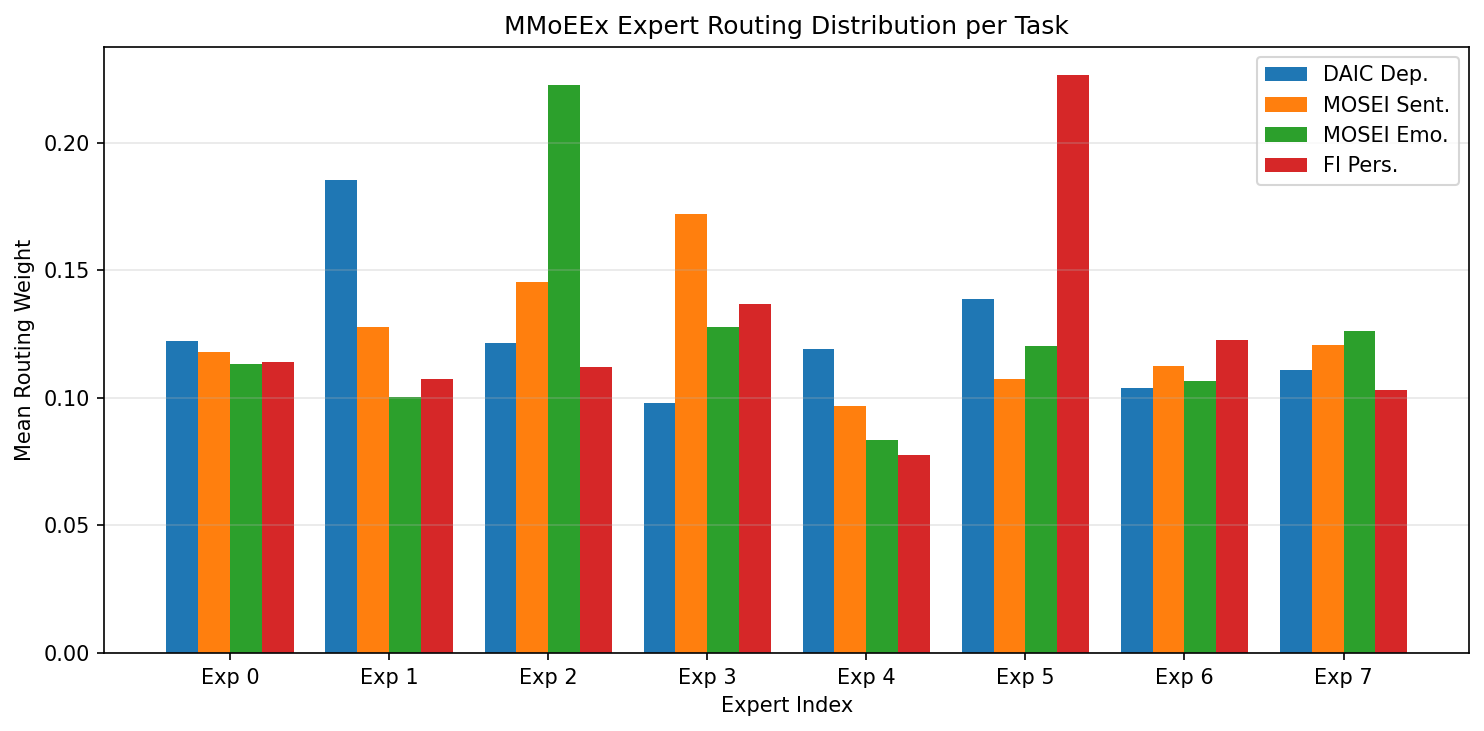
\includegraphics[width=0.9\columnwidth]{figures/expert_distribution.png}
\caption{Mean MMoEEx routing weight per expert and task (non-graph baseline). Rows/legend are tasks; columns are the 8 experts.}
\label{fig:expert_distribution}
\end{figure}

\section{Explainability Case Studies}
\label{sec:xai_supp}

Beyond the routing-performance question, the main paper's Introduction motivates two further, separately-evaluated hypotheses: that mental health assessment can be made more transparent by characterizing depression jointly with sentiment, emotion, and personality rather than in isolation, and that a graph over similar individuals can give both a visual and a machine-readable account of what informed a prediction. This section reports both.

\subsection{Multi-Construct Characterization}

For 9 case studies (3 per dataset), we pass the same sample's shared representation through all four task heads — not only the head matching its own source dataset — producing a depression probability, sentiment score, six emotion probabilities, and five personality-trait scores for the same person in one forward pass. On a representative positive-sentiment MOSEI case, the profile is internally coherent: happiness probability 0.89, sentiment score $+0.62$, with sadness/anger/fear all below 0.09 — a plausible joint characterization rather than four unrelated numbers. Related work explicitly separating personality-trait context from acute depression symptoms in an interpretable graph model \citep{vyalla2026psygat} supports this direction.

\subsection{Graph-Based Explanation}

For each case study we generate a visual record (SHAP per-modality beeswarm plot, GNNExplainer-style subgraph diagram \citep{gnnexplainer2019}, and a GraphXAIN-style \citep{cedro2024graphxain} natural-language narrative panel, Figure~\ref{fig:graphxain_supp}) and a machine-readable record (SHAP values, top-$k$ neighbour identities and cosine distances, expert routing weights, the multi-construct profile, and counterfactual/perturbation deltas). The narrative is generated by prompting an LLM (Mistral-7B) with the SHAP values, subgraph structure, and sample metadata, used purely as \emph{post-hoc} explanation of an independently-computed prediction — not as reasoning inserted into the prediction pipeline itself. This distinction matters: chain-of-thought-style reasoning improves mental-health text classification when used to produce the prediction \citep{patil2025cognitivemental}, but can be unfaithful or reduce reliability when embedded in the clinical decision itself \citep{wu2025cotfails}.

\begin{figure}[t]
\centering

\includegraphics[width=0.9\columnwidth]{figures/mosei_graphxain_panel.png}
\caption{GraphXAIN-style narrative panel for a representative MOSEI case, combining SHAP attribution, subgraph structure, and sample metadata into a post-hoc natural-language explanation.}
\label{fig:graphxain_supp}
\end{figure}

Every SHAP, perturbation, and counterfactual value must be computed under each sample's own dataset-native routing (main paper, Section 3): DAIC is evaluated text-only and FI video-only, so a modality outside a dataset's native routing shows \emph{exactly} zero attribution, not a small residual. Across 90 perturbation tests, only 47 are non-zero, exactly matching each sample's routing; the remaining 43 are exactly zero rather than merely small. This is a stronger faithfulness check than a ranking comparison: it directly confirms the explanation pipeline reflects each dataset's real computation.

\begin{figure}[t]
\centering
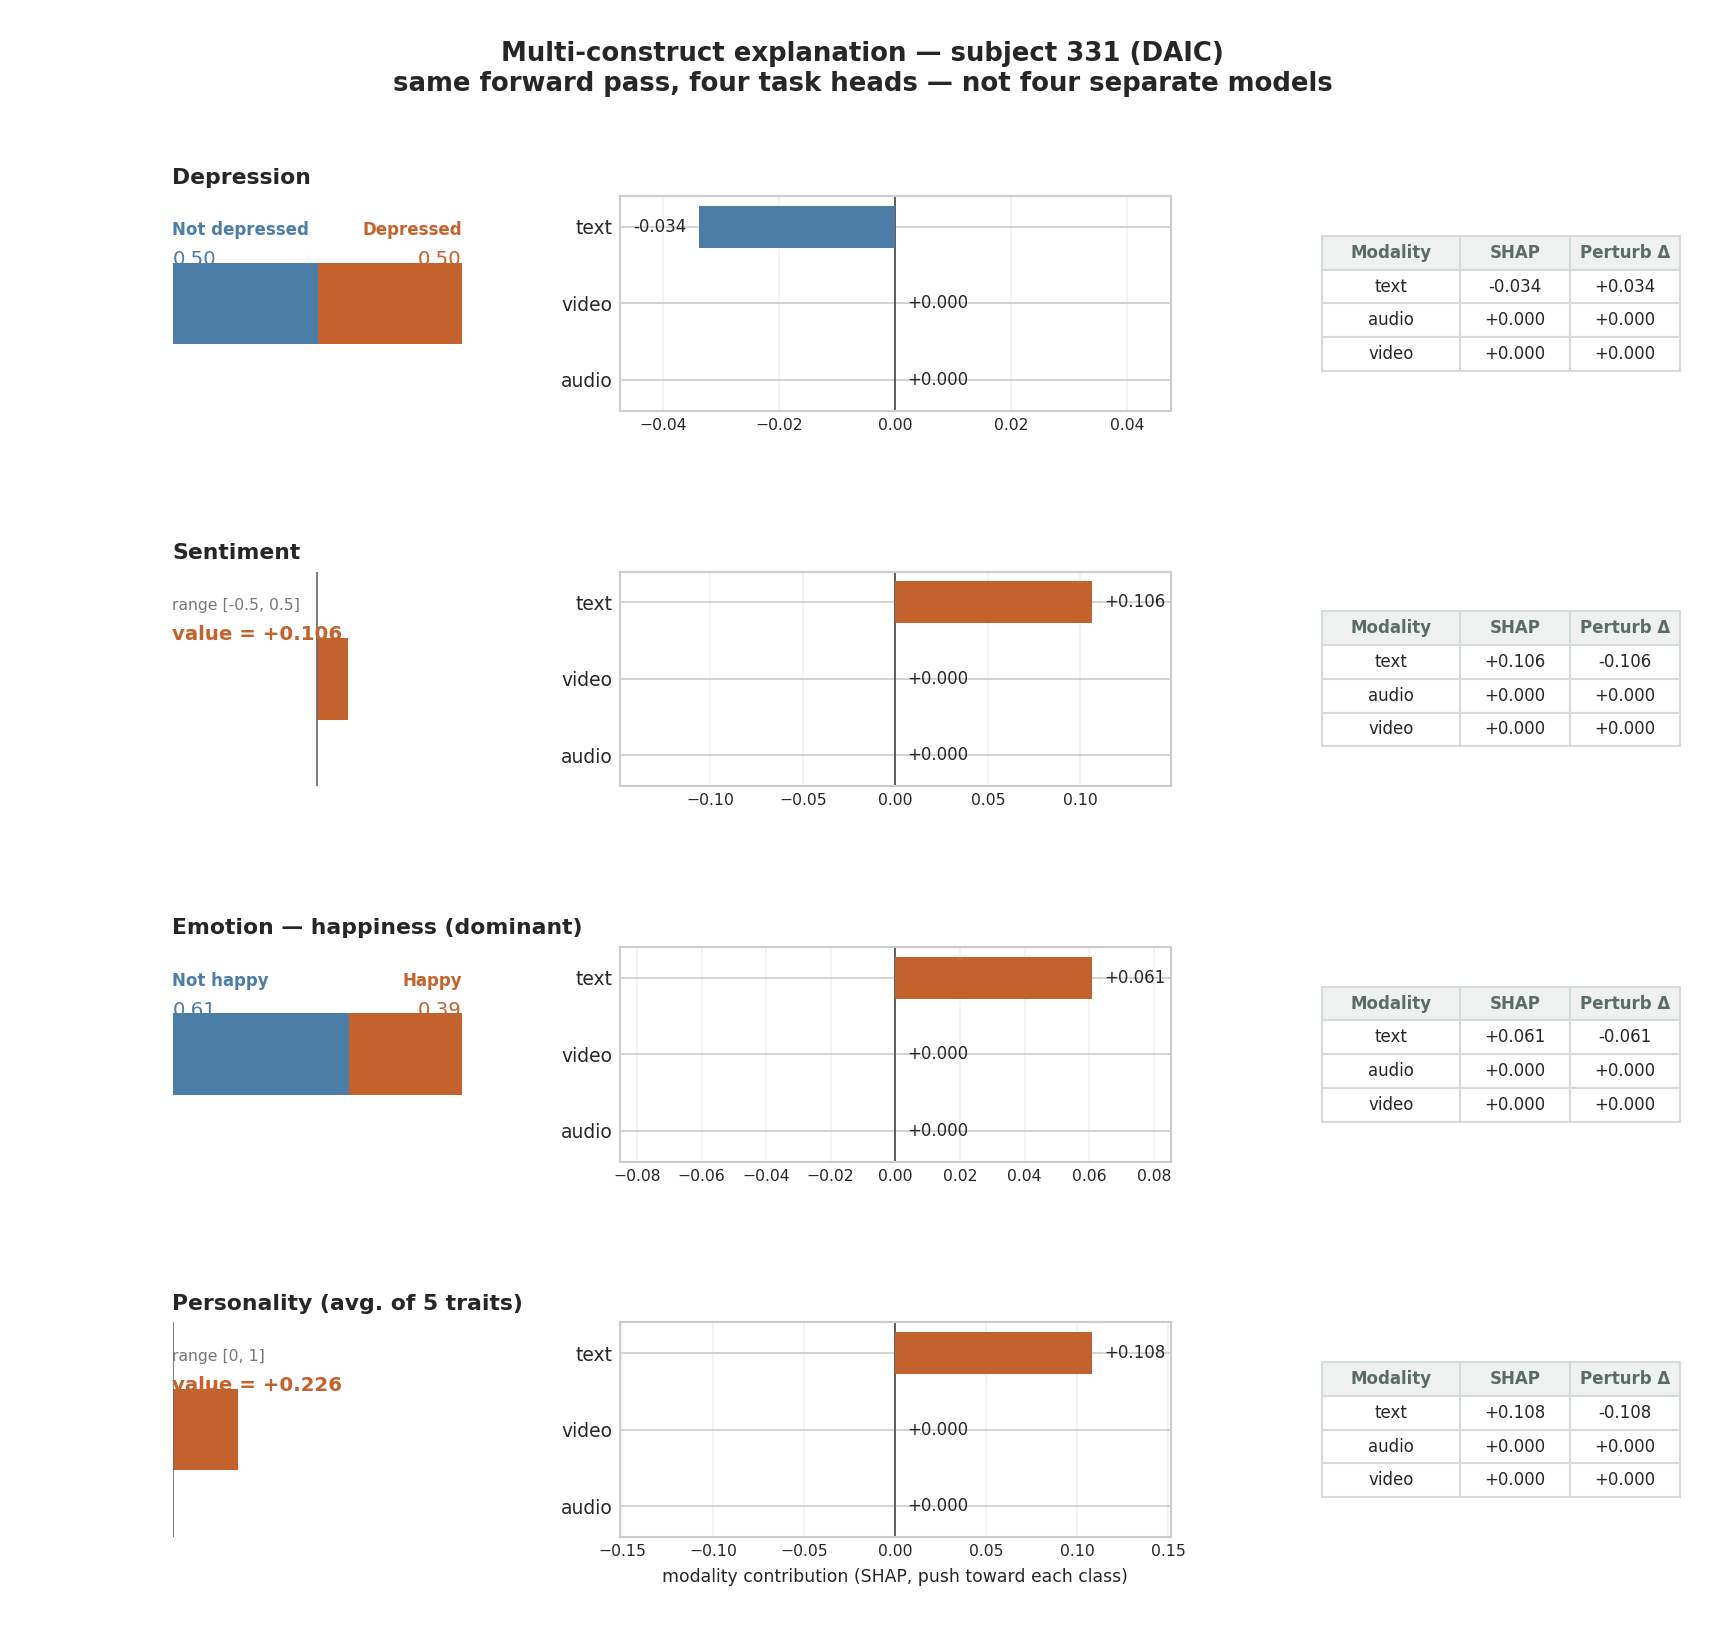
\includegraphics[width=0.9\columnwidth]{figures/daic_multi_construct_force.png}
\caption{Multi-construct force plot: one DAIC subject explained through all four task heads in a single figure. Audio and video read exactly zero on every row, visualizing DAIC's text-only routing directly rather than leaving it implicit.}
\label{fig:force_panel_supp}
\end{figure}

The explanation graph is built on the model's own trained fused representation rather than raw concatenated features, so reported neighbours are the ones the router and task heads actually operate on. This does not, however, improve DAIC label homophily: on the same 35 DAIC validation samples used for the main paper's homophily diagnostic, label agreement is 0.577 for raw features, 0.537 for random pairing, and 0.463 (below random) for the trained representation, since task-supervised training optimizes for the final decision boundary rather than for preserving neighbourhood structure. DAIC subgraph explanations should be read as faithful to the model's own computation, without a validated claim that the shown neighbours are similar in a depression-relevant sense; MOSEI and FI do not share this limitation, consistent with the main paper's homophily diagnostic finding real label signal for those tasks.




\bibliography{references/references}
\end{document}
